\documentclass[11pt,a4paper]{report}
\usepackage[textwidth=37em,vmargin=30mm]{geometry}
\usepackage{calc,xunicode,amsmath,amssymb,paralist,enumitem,tabu,booktabs,datetime2,xeCJK,xeCJKfntef,listings}
\usepackage{tocloft,fancyhdr,tcolorbox,xcolor,graphicx,eso-pic,xltxtra,xelatexemoji}

\newcommand{\envyear}[0]{2024}
\newcommand{\envdatestr}[0]{2024-11-15}
\newcommand{\envfinaldir}[0]{webdb/2024/20241115/final}

\usepackage[hidelinks]{hyperref}
\hypersetup{
    colorlinks=false,
    pdfpagemode=FullScreen,
    pdftitle={Web Digest - \envdatestr}
}

\setlength{\cftbeforechapskip}{10pt}
\renewcommand{\cftchapfont}{\rmfamily\bfseries\large\raggedright}
\setlength{\cftbeforesecskip}{2pt}
\renewcommand{\cftsecfont}{\sffamily\small\raggedright}

\setdefaultleftmargin{2em}{2em}{1em}{1em}{1em}{1em}

\usepackage{xeCJK,xeCJKfntef}
\xeCJKsetup{PunctStyle=plain,RubberPunctSkip=false,CJKglue=\strut\hskip 0pt plus 0.1em minus 0.05em,CJKecglue=\strut\hskip 0.22em plus 0.2em}
\XeTeXlinebreaklocale "zh"
\XeTeXlinebreakskip = 0pt


\setmainfont{Brygada 1918}
\setromanfont{Brygada 1918}
\setsansfont{IBM Plex Sans}
\setmonofont{JetBrains Mono NL}
\setCJKmainfont{Noto Serif CJK SC}
\setCJKromanfont{Noto Serif CJK SC}
\setCJKsansfont{Noto Sans CJK SC}
\setCJKmonofont{Noto Sans CJK SC}

\setlength{\parindent}{0pt}
\setlength{\parskip}{8pt}
\linespread{1.15}

\lstset{
	basicstyle=\ttfamily\footnotesize,
	numbersep=5pt,
	backgroundcolor=\color{black!5},
	showspaces=false,
	showstringspaces=false,
	showtabs=false,
	tabsize=2,
	captionpos=b,
	breaklines=true,
	breakatwhitespace=true,
	breakautoindent=true,
	linewidth=\textwidth
}






\newcommand{\coverpic}[2]{
    % argv: itemurl, authorname
    Cover photo by #2~~(\href{#1}{#1})
}
\newcommand{\makeheader}[0]{
    \begin{titlepage}
        % \newgeometry{hmargin=15mm,tmargin=21mm,bmargin=12mm}
        \begin{center}
            
            \rmfamily\scshape
            \fontspec{BaskervilleF}
            \fontspec{Old Standard}
            \fontsize{59pt}{70pt}\selectfont
            WEB\hfill DIGEST
            
            \vfill
            % \vskip 30pt
            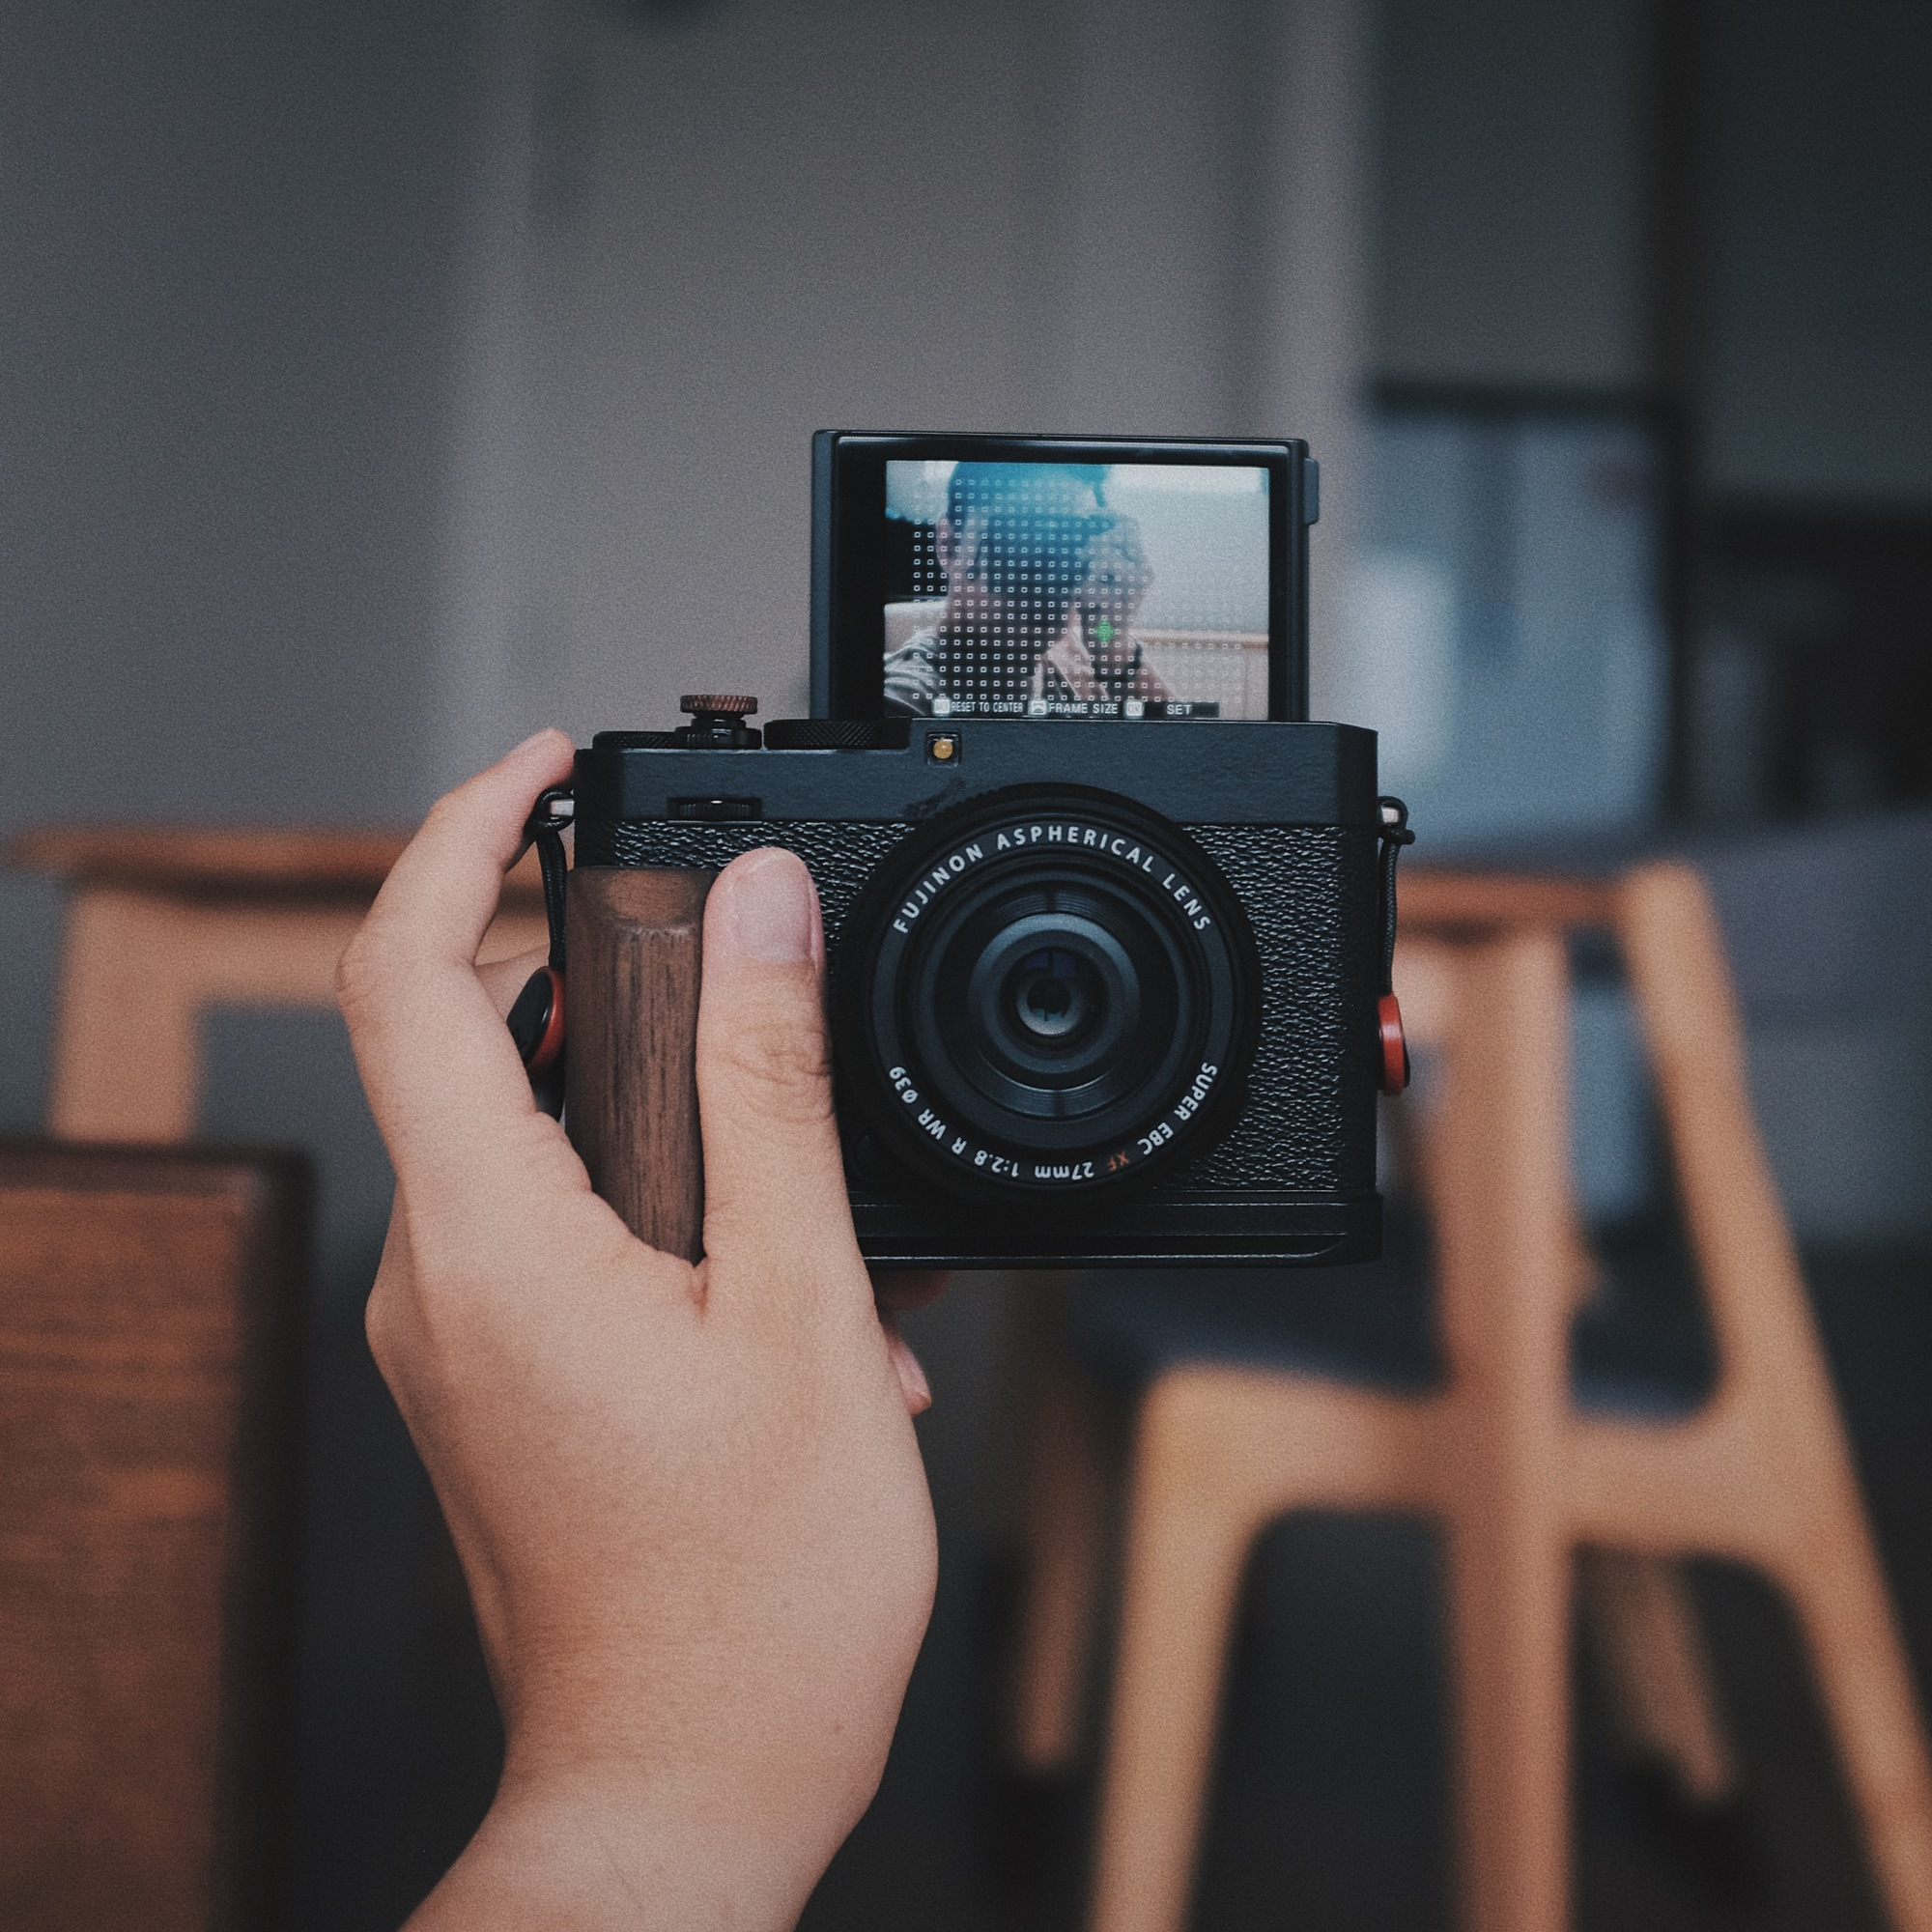
\includegraphics[width=\linewidth]{\envfinaldir/coverpic-prod.jpg}\par
            % \vskip 30pt
            \vfill

            \normalsize\rmfamily\scshape
            \copyright{} The Web Digest Project \hfill\large \envdatestr
        \end{center}
    \end{titlepage}
    % \restoregeometry
}
\newcommand{\simplehref}[1]{%
    \textcolor{blue!80!green}{\href{#1}{#1}}%
}
\renewcommand{\contentsname}{\center\Huge\sffamily\bfseries Contents\par\vskip 20pt}
\newcounter{ipartcounter}
\setcounter{ipartcounter}{0}
\newcommand{\ipart}[1]{
    % \vskip 20pt
    \clearpage
    \stepcounter{ipartcounter}
    \phantomsection
    \addcontentsline{toc}{chapter}{#1}
    % \begin{center}
    %     \Huge
    %     \sffamily\bfseries
    %     #1
    % \end{center}
    % \vskip 20pt plus 7pt
}
\newcounter{ichaptercounter}
\setcounter{ichaptercounter}{0}
\newcommand{\ichapter}[1]{
    % \vskip 20pt
    \clearpage
    \stepcounter{ichaptercounter}
    \phantomsection
    \addcontentsline{toc}{section}{\numberline{\arabic{ichaptercounter}}#1}
    \begin{center}
        \Huge
        \sffamily\bfseries
        #1
    \end{center}
    \vskip 20pt plus 7pt
}
\newcommand{\entrytitlefont}[1]{\subsection*{\raggedright\Large\sffamily\bfseries#1}}
\newcommand{\entryitemGeneric}[2]{
    % argv: title, url
    \parbox{\linewidth}{
        \entrytitlefont{#1}\par\vskip 5pt
        \footnotesize\ttfamily\mdseries
        \simplehref{#2}
    }\vskip 11pt plus 11pt minus 1pt
}
\newcommand{\entryitemGithub}[3]{
    % argv: title, url, desc
    \parbox{\linewidth}{
        \entrytitlefont{#1}\par\vskip 5pt
        \footnotesize\ttfamily\mdseries
        \simplehref{#2}\par\vskip 5pt
        \small\rmfamily\mdseries#3
    }\vskip 11pt plus 11pt minus 1pt
}
\newcommand{\entryitemAp}[3]{
    % argv: title, url, desc
    \parbox{\linewidth}{
        \entrytitlefont{#1}\par\vskip 5pt
        \footnotesize\ttfamily\mdseries
        \simplehref{#2}\par\vskip 5pt
        \small\rmfamily\mdseries#3
    }\vskip 11pt plus 11pt minus 1pt
}
\newcommand{\entryitemHackernews}[3]{
    % argv: title, hnurl, rawurl
    % \parbox{\linewidth}{
    %     \entrytitlefont{#1}\par\vskip 5pt
    %     \footnotesize\ttfamily\mdseries
    %     \simplehref{#3}\par
    %     \textcolor{black!50}{\href{#2}{#2}}
    % }\vskip 11pt plus 11pt minus 1pt
    \begin{minipage}{\linewidth}
            \entrytitlefont{#1}\par\vskip 5pt
            \footnotesize\ttfamily\mdseries
            \simplehref{#3}\par
            \textcolor{black!50}{\href{#2}{#2}}
    \end{minipage}\par\vskip 11pt plus 11pt minus 1pt
}







\begin{document}

\makeheader

\tableofcontents\clearpage




\ipart{Developers}
\ichapter{Hacker News}
\entryitemTwoLinks{Analysis of economic and productivity losses caused by cookie banners in Europe}{https://news.ycombinator.com/item?id=42141843}{https://legiscope.com/blog/hidden-productivity-drain-cookie-banners.html}

\entryitemTwoLinks{Red Hat to contribute container tech (Podman, bootc, ComposeFS...) to CNCF}{https://news.ycombinator.com/item?id=42139044}{https://www.redhat.com/en/blog/red-hat-contribute-comprehensive-container-tools-collection-cloud-native-computing-foundation}

\entryitemTwoLinks{Something weird is happening with LLMs and Chess}{https://news.ycombinator.com/item?id=42138276}{https://dynomight.net/chess/}

\entryitemTwoLinks{Daisy, an AI granny wasting scammers' time}{https://news.ycombinator.com/item?id=42138115}{https://news.virginmediao2.co.uk/o2-unveils-daisy-the-ai-granny-wasting-scammers-time/}

\entryitemTwoLinks{The letter ℘: name and origin? (2017)}{https://news.ycombinator.com/item?id=42137818}{https://mathoverflow.net/questions/278130/the-letter-wp-name-origin}

\entryitemTwoLinks{AI makes tech debt more expensive}{https://news.ycombinator.com/item?id=42137527}{https://www.gauge.sh/blog/ai-makes-tech-debt-more-expensive}

\entryitemTwoLinks{On Building Git for Lawyers}{https://news.ycombinator.com/item?id=42137391}{https://jordanbryan.substack.com/p/on-building-git-for-lawyers}

\entryitemTwoLinks{The barriers to AI engineering are crumbling fast}{https://news.ycombinator.com/item?id=42136711}{https://blog.helix.ml/p/we-can-all-be-ai-engineers}

\entryitemTwoLinks{Why is it so hard to find a job now? Enter Ghost Jobs}{https://news.ycombinator.com/item?id=42136469}{https://arxiv.org/abs/2410.21771}

\entryitemTwoLinks{PyPI now supports digital attestations}{https://news.ycombinator.com/item?id=42136375}{https://blog.pypi.org/posts/2024-11-14-pypi-now-supports-digital-attestations/}

\entryitemTwoLinks{The Onion wins Alex Jones' Infowars in bankruptcy auction}{https://news.ycombinator.com/item?id=42136327}{https://www.nbcnews.com/news/us-news/onion-wins-alex-jones-infowars-bankruptcy-auction-rcna179936}

\entryitemTwoLinks{The Onion buys Infowars}{https://news.ycombinator.com/item?id=42136259}{https://www.nytimes.com/2024/11/14/business/media/alex-jones-infowars-the-onion.html}

\entryitemTwoLinks{A memory leak in Apple's Network Extension framework}{https://news.ycombinator.com/item?id=42136136}{https://obdev.at/blog/a-memory-leak-in-apples-network-extension-framework/}

\entryitemTwoLinks{An analysis of the Keycloak authentication system}{https://news.ycombinator.com/item?id=42136000}{https://security.humanativaspa.it/an-analysis-of-the-keycloak-authentication-system/}

\entryitemTwoLinks{MomBoard: E-ink display for a parent with amnesia}{https://news.ycombinator.com/item?id=42135520}{https://jan.miksovsky.com/posts/2024/11-12-momboard}

\entryitemTwoLinks{SQLite Index Visualization}{https://news.ycombinator.com/item?id=42134964}{https://mrsuh.com/articles/2024/sqlite-index-visualization-structure/}

\entryitemTwoLinks{DeepL Voice: Real-time voice translations for global collaboration}{https://news.ycombinator.com/item?id=42134475}{https://www.deepl.com/en/products/voice}

\entryitemTwoLinks{Interview with gwern}{https://news.ycombinator.com/item?id=42134315}{https://www.dwarkeshpatel.com/p/gwern-branwen}

\entryitemTwoLinks{Lessons from my first exit}{https://news.ycombinator.com/item?id=42133864}{https://mtlynch.io/lessons-from-my-first-exit/}

\entryitemTwoLinks{I Followed the Official AWS Amplify Guide and Was Charged \$1,100}{https://news.ycombinator.com/item?id=42133700}{https://elliott-king.github.io/2024/10/amplify-overcharge/}\ichapter{Phoronix}
\entryitemGeneric{\hskip 0pt{}Khronos SYCL Being Updated To Increase Appeal For HPC \& Scientific Computing}{https://www.phoronix.com/news/Khronos-SYCL-HPC-SC24}

\entryitemGeneric{\hskip 0pt{}OpenMP 6.0 Released With An Emphasis On Easier Parallel Programming}{https://www.phoronix.com/news/OpenMP-6.0-Released}

\entryitemGeneric{\hskip 0pt{}Upstream Linux Developers Take Aim At TUXEDO's Out-Of-Tree GPLv3 Drivers}{https://www.phoronix.com/news/TUXEDO-Drivers-Taint-Patches}

\entryitemGeneric{\hskip 0pt{}Supermicro H13SSL-N For AMD EPYC 9005 "Turin" 1P Servers}{https://www.phoronix.com/review/supermicro-h13ssln-epyc-turin}

\entryitemGeneric{\hskip 0pt{}Red Hat Enterprise Linux 10 Enters Beta With Many New Features \& Updates}{https://www.phoronix.com/news/Red-Hat-RHEL-10-Beta}

\entryitemGeneric{\hskip 0pt{}AMD 3D V-Cache Optimizer Driver To Be Merged For Linux 6.13}{https://www.phoronix.com/news/AMD-3DV-Optimizer-Linux-6.13}

\entryitemGeneric{\hskip 0pt{}Linux 6.13 To Tune Intel Granite Rapids For Better Performance Out-Of-The-Box}{https://www.phoronix.com/news/Linux-6.13-Granite-Rapids-EPP}

\entryitemGeneric{\hskip 0pt{}Linux To Allow Disabling TPM PCR Integrity Protection Due To Performance Bottleneck}{https://www.phoronix.com/news/Linux-TPM-Disable-PCR-Integrity}

\entryitemGeneric{\hskip 0pt{}Intel Touch Host Controller "THC" Driver Support Being Worked On For Linux}{https://www.phoronix.com/news/Intel-Touch-Host-Controller}


\ipart{Developers~~~~(zh-Hans)}
\ichapter{Solidot}
\entryitemGeneric{\hskip 0pt{}洋葱新闻拍下了 InfoWars}{https://www.solidot.org/story?sid=79778}

\entryitemGeneric{\hskip 0pt{}意大利出人意料的成为间谍软件的主要供应国}{https://www.solidot.org/story?sid=79777}

\entryitemGeneric{\hskip 0pt{}AI 只能完成高等数学新测试问题的不到 2\%}{https://www.solidot.org/story?sid=79776}

\entryitemGeneric{\hskip 0pt{}GOG 宣布了经典游戏的保存计划}{https://www.solidot.org/story?sid=79775}

\entryitemGeneric{\hskip 0pt{}Steam 停止支持 Windows 7 和 Windows 8}{https://www.solidot.org/story?sid=79774}

\entryitemGeneric{\hskip 0pt{}微软证实在开发掌机}{https://www.solidot.org/story?sid=79773}

\entryitemGeneric{\hskip 0pt{}微软宣布 .NET 9}{https://www.solidot.org/story?sid=79772}

\entryitemGeneric{\hskip 0pt{}AMD 裁员 4\%}{https://www.solidot.org/story?sid=79771}

\entryitemGeneric{\hskip 0pt{}Bluesky 用户突破 1500 万}{https://www.solidot.org/story?sid=79770}

\entryitemGeneric{\hskip 0pt{}苹果高管为 M4 Mac mini 电源按钮位置辩护}{https://www.solidot.org/story?sid=79769}

\entryitemGeneric{\hskip 0pt{}Discord 泄密者Jack Teixeira 被判 15 年}{https://www.solidot.org/story?sid=79768}

\entryitemGeneric{\hskip 0pt{}VMware Workstation Pro 对商业使用免费}{https://www.solidot.org/story?sid=79767}

\entryitemGeneric{\hskip 0pt{}SpaceX 计划测试 Starship 在轨加油 }{https://www.solidot.org/story?sid=79766}

\entryitemGeneric{\hskip 0pt{}微软 Edge 再次试图自动导入 Chrome 数据}{https://www.solidot.org/story?sid=79765}

\entryitemGeneric{\hskip 0pt{}AI大神李继刚空降PEC大会,解锁你的专属}{https://www.solidot.org/story?sid=79764}

\entryitemGeneric{\hskip 0pt{}中国品牌电视机占日本五成市场份额}{https://www.solidot.org/story?sid=79763}

\entryitemGeneric{\hskip 0pt{}额外一年的教育对大脑结构变化没有产生长期影响}{https://www.solidot.org/story?sid=79762}

\entryitemGeneric{\hskip 0pt{}Red Hat 收购 Neural Magic,将开源其技术 }{https://www.solidot.org/story?sid=79761}

\entryitemGeneric{\hskip 0pt{}木星质量双星如何形成}{https://www.solidot.org/story?sid=79760}

\entryitemGeneric{\hskip 0pt{}中国在珠海航展展示了新隐形战斗机 }{https://www.solidot.org/story?sid=79759}\ichapter{V2EX}
\entryitemGeneric{\hskip 0pt{}[职场话题] 一个独立开发者 是否需要掌握 ui 设计}{https://www.v2ex.com/t/1089704}

\entryitemGeneric{\hskip 0pt{}[问与答] 2024 年求推荐性价比高的头戴式耳机,编程或者健身房场景下使用}{https://www.v2ex.com/t/1089703}

\entryitemGeneric{\hskip 0pt{}[问与答] 求推荐视频自媒体工具}{https://www.v2ex.com/t/1089702}

\entryitemGeneric{\hskip 0pt{}[Apple] M1-M4 CPU/GPU 对比表格}{https://www.v2ex.com/t/1089701}

\entryitemGeneric{\hskip 0pt{}[Apple] 有任何可能把 M1 iMac 当作其他 Mac 电脑的显示器使用吗?}{https://www.v2ex.com/t/1089700}

\entryitemGeneric{\hskip 0pt{}[问与答] Firefox for Android 的域名栏识别问题算 BUG 吗?}{https://www.v2ex.com/t/1089699}

\entryitemGeneric{\hskip 0pt{}[问与答] 求推荐长辈用手机}{https://www.v2ex.com/t/1089698}

\entryitemGeneric{\hskip 0pt{}[Linux] 什么情况下才会自己编译内核?}{https://www.v2ex.com/t/1089695}

\entryitemGeneric{\hskip 0pt{}[macOS] macOS 设置 ThunderBolt Bridge 的状态 BUG 'unknown state'}{https://www.v2ex.com/t/1089694}

\entryitemGeneric{\hskip 0pt{}[Apple] M4 Mac Mini 真棒,特别是自带音箱这点,所以我想当蓝牙音箱用}{https://www.v2ex.com/t/1089693}

\entryitemGeneric{\hskip 0pt{}[Apple] 买了一个 Mac mini M4, 3677,用的太爽了,比之前丐版 M2。现在有升级冲动,有优惠, Mac mini M4 24G 512 需要 6000,朋友们,该换吗?}{https://www.v2ex.com/t/1089692}

\entryitemGeneric{\hskip 0pt{}[分享创造] 一枚想出海的程序媛的第一次尝试}{https://www.v2ex.com/t/1089690}

\entryitemGeneric{\hskip 0pt{}[问与答] 双十一买了两台手机,我应该留哪个?}{https://www.v2ex.com/t/1089688}

\entryitemGeneric{\hskip 0pt{}[Apple] 突然发现, final cut pro 居然是 macos 独立的, iPad 上的居然要收费,不能共享}{https://www.v2ex.com/t/1089687}

\entryitemGeneric{\hskip 0pt{}[问与答] 感觉 hoppscotch 的文档中自托管部分,是故意写的很坑,不想让人自建的......}{https://www.v2ex.com/t/1089686}

\entryitemGeneric{\hskip 0pt{}[NAS] Mac 读写 nas 比 win 慢是正常吗}{https://www.v2ex.com/t/1089685}

\entryitemGeneric{\hskip 0pt{}[职场话题] 学生一名,徘徊在不断学技术和害怕技术不达要求没公司要}{https://www.v2ex.com/t/1089684}

\entryitemGeneric{\hskip 0pt{}[Apple] Apple One 美区全家桶组队}{https://www.v2ex.com/t/1089683}

\entryitemGeneric{\hskip 0pt{}[Mac mini] 请问 mac mini 只有键盘怎么连接蓝牙鼠标}{https://www.v2ex.com/t/1089682}

\entryitemGeneric{\hskip 0pt{}[小米] 小米 15/hyperOS 2.0 打开 FCM 通知}{https://www.v2ex.com/t/1089681}

\entryitemGeneric{\hskip 0pt{}[问与答] 有什么推荐的轻 blog}{https://www.v2ex.com/t/1089680}

\entryitemGeneric{\hskip 0pt{}[上海] 出升降桌和人体工学椅}{https://www.v2ex.com/t/1089679}

\entryitemGeneric{\hskip 0pt{}[问与答] mac 鼠标不跟手}{https://www.v2ex.com/t/1089678}

\entryitemGeneric{\hskip 0pt{}[云计算] 腾讯云又一个可用区下线了}{https://www.v2ex.com/t/1089675}

\entryitemGeneric{\hskip 0pt{}[问与答] 大华的 sdk 一个头文件 130,000 行}{https://www.v2ex.com/t/1089674}

\entryitemGeneric{\hskip 0pt{}[问与答] IOS18 无密码取证是真的吗?这个视频}{https://www.v2ex.com/t/1089673}

\entryitemGeneric{\hskip 0pt{}[分享创造] 谁做过 AI 编程 用 bolt.new 或者 v0.dev 做个在线词典和翻译的网站?}{https://www.v2ex.com/t/1089672}

\entryitemGeneric{\hskip 0pt{}[问与答] 感觉有双无形的手故意把我困在一个圈里,怎么出这个圈?}{https://www.v2ex.com/t/1089670}

\entryitemGeneric{\hskip 0pt{}[问与答] 教教我怎么给小火箭写配置规则}{https://www.v2ex.com/t/1089669}

\entryitemGeneric{\hskip 0pt{}[分享创造] 几分钟做了一个手机横屏时间显示}{https://www.v2ex.com/t/1089668}

\entryitemGeneric{\hskip 0pt{}[生活] 深圳安居房闲置怎么办}{https://www.v2ex.com/t/1089667}

\entryitemGeneric{\hskip 0pt{}[宽带症候群] PCDN 是真的毒瘤,一周刷了我 4T 多上行}{https://www.v2ex.com/t/1089666}

\entryitemGeneric{\hskip 0pt{}[Android] 如何实现在游戏期间对后台进程进行额外的限制?}{https://www.v2ex.com/t/1089665}

\entryitemGeneric{\hskip 0pt{}[MacBook] AIDente 这个软件大家觉得有用么?}{https://www.v2ex.com/t/1089663}

\entryitemGeneric{\hskip 0pt{}[程序员] 大家有 Aha! moment(顿悟时刻)吗?}{https://www.v2ex.com/t/1089661}

\entryitemGeneric{\hskip 0pt{}[macOS] playcover 安装闲鱼,打开之后卡在初始界面}{https://www.v2ex.com/t/1089660}

\entryitemGeneric{\hskip 0pt{}[问与答] 28 岁,腰间盘突出,应该怎么恢复?}{https://www.v2ex.com/t/1089659}

\entryitemGeneric{\hskip 0pt{}[问与答] [win 文件丢失] 这问题真就无解么?}{https://www.v2ex.com/t/1089658}

\entryitemGeneric{\hskip 0pt{}[问与答] 求教:预算 6k 买哪款安卓手机?(女士用。请勿推荐 iPhone ,华为及荣耀暂不考虑。其他需求见正文)多谢多谢}{https://www.v2ex.com/t/1089657}

\entryitemGeneric{\hskip 0pt{}[程序员] 发现一个不错的简历生成器}{https://www.v2ex.com/t/1089656}

\entryitemGeneric{\hskip 0pt{}[macOS] LSD(Launch Service Daemon)硬盘持续写入问题}{https://www.v2ex.com/t/1089655}

\entryitemGeneric{\hskip 0pt{}[分享创造] 体验了一下现在 AI 对于小型项目的编码能力}{https://www.v2ex.com/t/1089654}

\entryitemGeneric{\hskip 0pt{}[问与答] 为什么``即刻''的内容质量很高,但评论互动极少?}{https://www.v2ex.com/t/1089653}

\entryitemGeneric{\hskip 0pt{}[NAS] 极空间是不是不支持自动把文件夹内容变更同步到云盘里}{https://www.v2ex.com/t/1089652}

\entryitemGeneric{\hskip 0pt{}[宽带症候群] 武汉电信 5g 239-80,再开超千兆提速包 2000M 上传 100-120M}{https://www.v2ex.com/t/1089651}

\entryitemGeneric{\hskip 0pt{}[分享创造] 电脑 NTQQ 炫酷消息插件}{https://www.v2ex.com/t/1089650}

\entryitemGeneric{\hskip 0pt{}[问与答] 杭州辞职之后,你们的社保医保怎么解决的}{https://www.v2ex.com/t/1089649}

\entryitemGeneric{\hskip 0pt{}[问与答] 哪个 orm 支持 PostgreSQL 的 range 类型? typescript 语言}{https://www.v2ex.com/t/1089648}

\entryitemGeneric{\hskip 0pt{}[MacBook Pro] 笔记本选购求建议,编程建模渲染}{https://www.v2ex.com/t/1089647}

\entryitemGeneric{\hskip 0pt{}[电动汽车] 问界汽车居然不对电路板做防水保护,难受了}{https://www.v2ex.com/t/1089646}


\ipart{Generic News}
\ichapter{Reuters}
\entryitemWithDescription{\hskip 0pt{}Israeli anthem booed, brief scuffles at France game}{https://www.reuters.com/sports/soccer/israeli-anthem-booed-brief-scuffles-france-game-2024-11-14/}{Some French fans booed the Israeli national anthem and there were minor scuffles inside a sparsely-attended Stade de France on Wednesday for a Nations League game overshadowed by frictions around the Gaza...}

\entryitemWithDescription{\hskip 0pt{}North Korea leader Kim orders mass production of suicide drones, Yonhap says}{https://www.reuters.com/world/asia-pacific/north-korea-leader-kim-orders-mass-production-suicide-drones-yonhap-says-2024-11-14/}{North Korean leader Kim Jong Un guided a test of suicide drones and ordered a mass production of the aerial weapon, Yonhap news agency said on...}

\entryitemWithDescription{\hskip 0pt{}Russian drone attack kills one, damages energy installations in Ukraine's Odesa}{https://www.reuters.com/world/europe/russian-drone-attack-damages-energy-installations-ukraines-odesa-2024-11-14/}{Russian drones struck a residential building and energy installations on Thursday evening in and near Ukraine\textquotesingle s Black Sea port of Odesa, killing one person, injuring at least two and knocking out a boiler plant used for...}

\entryitemWithDescription{\hskip 0pt{}Mexico's Sinaloa state probing killing of 14 people, prosecutors say}{https://www.reuters.com/world/americas/mexicos-sinaloa-state-probing-killing-14-people-prosecutors-say-2024-11-14/}{The prosecutor\textquotesingle s office of Mexico\textquotesingle s Sinaloa state is investigating the killing of some 14 people, whose bodies were found around the city of Culiacan, it said in a statement on...}

\entryitemWithDescription{\hskip 0pt{}Israeli strike kills 12 after hitting civil defence centre in Lebanon's Baalbek, governor tells Reuters}{https://www.reuters.com/world/middle-east/israeli-strike-kills-12-after-hitting-civil-defence-centre-lebanons-baalbek-2024-11-14/}{An Israeli strike killed 12 people after it hit a civil defence centre in Lebanon\textquotesingle s city of Baalbek on Thursday, the regional governor told Reuters adding that rescue operations were...}

\entryitemWithDescription{\hskip 0pt{}Nicaragua expels lead bishop in crackdown on Catholic Church}{https://www.reuters.com/world/americas/nicaragua-expels-lead-bishop-crackdown-catholic-church-2024-11-14/}{Nicaragua has expelled Bishop Carlos Herrera, the head of the country\textquotesingle s episcopal conference, a lawyer tied to the Catholic Church told Reuters on Thursday, amid an extended state crackdown targeting the...}

\entryitemWithDescription{\hskip 0pt{}Israeli strike kills 6 people, including 4 medics, in southern Lebanon, ministry says}{https://www.reuters.com/world/middle-east/israeli-strike-kills-6-people-including-4-medics-southern-lebanon-ministry-says-2024-11-14/}{An Israeli strike killed six people, including four medics, in the village of Arab Salim in southern Lebanon on Thursday, the health ministry said in a...}

\entryitemWithDescription{\hskip 0pt{}Scant crowd and heavy security at Stade de France for Israel game}{https://www.reuters.com/sports/soccer/scant-crowd-heavy-security-stade-de-france-israel-game-2024-11-14/}{Crowds were thin and security was heavy at the Stade de France for Les Bleus\textquotesingle{} Nations League game against Israel on Thursday after violence in Amsterdam last week around a Europa League match involving Maccabi Tel...}

\entryitemWithDescription{\hskip 0pt{}Austrian prosecutors ask parliament to lift far-right leader's immunity}{https://www.reuters.com/world/europe/austrian-prosecutors-ask-parliament-lift-far-right-leaders-immunity-2024-11-14/}{Austrian prosecutors have asked parliament to lift far-right leader Herbert Kickl\textquotesingle s immunity over an allegation that he committed perjury testifying to a parliamentary committee, the office of the lower house...}

\entryitemWithDescription{\hskip 0pt{}Democrats in Congress urge Biden to sanction Israelis over West Bank violence}{https://www.reuters.com/world/us/democrats-congress-urge-biden-sanction-israelis-over-west-bank-violence-2024-11-14/}{The letter said Israeli settlers have carried out over 1,270 recorded attacks in the West...}

\entryitemWithDescription{\hskip 0pt{}Israel will attack any attempt to bring arms to Hezbollah from Syria -army spokesperson}{https://www.reuters.com/world/middle-east/israel-will-attack-any-attempt-bring-arms-hezbollah-syria-army-spokesperson-2024-11-14/}{Israel will attack any attempt to bring weapons to Hezbollah from Syria, Israel\textquotesingle s military spokesperson said on...}

\entryitemWithDescription{\hskip 0pt{}Thousands protest in Vilnius against government party whose leader is on trial for antisemitism}{https://www.reuters.com/world/europe/thousands-protest-vilnius-against-government-party-whose-leader-is-trial-2024-11-14/}{More than 5,000 people protested next to the Lithuanian parliament on Thursday against election winners the Social Democrats entering into a parliamentary coalition with a party whose leader is on trial accused of antisemitic...}

\entryitemWithDescription{\hskip 0pt{}Global measles cases jumped in 2023 due to 'inadequate' vaccine coverage}{https://www.reuters.com/business/healthcare-pharmaceuticals/global-measles-cases-jumped-2023-due-inadequate-vaccine-coverage-2024-11-14/}{Measles cases rose 20\% last year, driven by a lack of vaccine coverage in the world\textquotesingle s poorest countries and those riddled with conflict, the World Health Organization and the U.S. Centers for Disease Control and...}






\clearpage
\leavevmode\vfill
\footnotesize

Copyright \copyright{} 2023-2024 Neruthes and other contributors.

This document is published with CC BY-NC-ND 4.0 license.

The entries listed in this newsletter may be copyrighted by their respective creators.

This newsletter is generated by the Web Digest project.

The newsletters are also delivered via Telegram channel \CJKunderline{\href{https://t.me/webdigestchannel}{https://t.me/webdigestchannel}}.\\
RSS feed is available at \CJKunderline{\href{https://webdigest.pages.dev/rss.xml}{https://webdigest.pages.dev/rss.xml}}.

This newsletter is available in PDF at
\CJKunderline{\href{https://webdigest.pages.dev/}{https://webdigest.pages.dev/}}.

The source code being used to generate this newsletter is available at\\
\CJKunderline{\href{https://github.com/neruthes/webdigest}{https://github.com/neruthes/webdigest}}.

This newsletter is also available in
\CJKunderline{\href{http://webdigest.pages.dev/readhtml/\envyear/WebDigest-20241115.html}{HTML}} and
\CJKunderline{\href{https://github.com/neruthes/webdigest/blob/master/markdown/\envyear/WebDigest-20241115.md}{Markdown}}.


\coverpic{https://unsplash.com/photos/a-woman-with-long-red-hair-wearing-a-white-dress-\_jdZk9J8phc}{Tiffany Longeway}


\end{document}
